\documentclass[11pt]{article}
\usepackage{geometry,marginnote} % Pour passer au format A4
\geometry{hmargin=1cm, vmargin=1cm} % 

% Page et encodage
\usepackage[T1]{fontenc} % Use 8-bit encoding that has 256 glyphs
\usepackage[english,french]{babel} % Français et anglais
\usepackage[utf8]{inputenc} 

\usepackage{lmodern,numprint}
\setlength\parindent{0pt}

% Graphiques
\usepackage{graphicx,float,grffile,units}
\usepackage{tikz,pst-eucl,pst-plot,pstricks,pst-node,pstricks-add,pst-fun,pgfplots} 

% Maths et divers
\usepackage{amsmath,amsfonts,amssymb,amsthm,verbatim}
\usepackage{multicol,enumitem,url,eurosym,gensymb,tabularx}

\DeclareUnicodeCharacter{20AC}{\euro}



% Sections
\usepackage{sectsty} % Allows customizing section commands
\allsectionsfont{\centering \normalfont\scshape}

% Tête et pied de page
\usepackage{fancyhdr} \pagestyle{fancyplain} \fancyhead{} \fancyfoot{}

\renewcommand{\headrulewidth}{0pt} % Remove header underlines
\renewcommand{\footrulewidth}{0pt} % Remove footer underlines

\newcommand{\horrule}[1]{\rule{\linewidth}{#1}} % Create horizontal rule command with 1 argument of height

\newcommand{\Pointilles}[1][3]{%
  \multido{}{#1}{\makebox[\linewidth]{\dotfill}\\[\parskip]
}}

\newtheorem{Definition}{Définition}

\usepackage{siunitx}
\sisetup{
    detect-all,
    output-decimal-marker={,},
    group-minimum-digits = 3,
    group-separator={~},
    number-unit-separator={~},
    inter-unit-product={~}
}

\setlength{\columnseprule}{1pt}

\begin{document}

\textbf{Nom, Prénom :} \hspace{8cm} \textbf{Classe :} \hspace{3cm} \textbf{Date :}\\

\vspace{-0.5cm} \begin{center}
  \textit{La valeur morale ne peut pas être remplacée par la valeur intelligence et j'ajouterai : Dieu merci !}  - \textbf{Albert Einstein}
\end{center}


\begin{minipage}[t]{0.3\textwidth}
\subsection*{Calcul des longueurs}

\begin{center}
  \begin{tabular}{|c|c|c|}
    \hline
    angle : $\alpha$ & opp : $\sin$ & adj : $\cos$\\  \hline
       0°          &           &          \\  \hline
       1°          &           &          \\  \hline
       5°          &           &          \\  \hline
       10°         &           &          \\  \hline
       20°         &           &          \\  \hline
       30°         &           &          \\  \hline
       40°         &           &          \\  \hline
       45°         &           &          \\  \hline
       50°         &           &          \\  \hline
       60°         &           &          \\  \hline
       70°         &           &          \\  \hline
       80°         &           &          \\  \hline
       85°         &           &          \\  \hline
       89°         &           &          \\  \hline
       90°         &           &          \\  \hline
  \end{tabular}
\end{center}

\end{minipage}
\begin{minipage}[t]{0.7\textwidth}

\begin{center}
\begin{figure}[H]
  \centering
  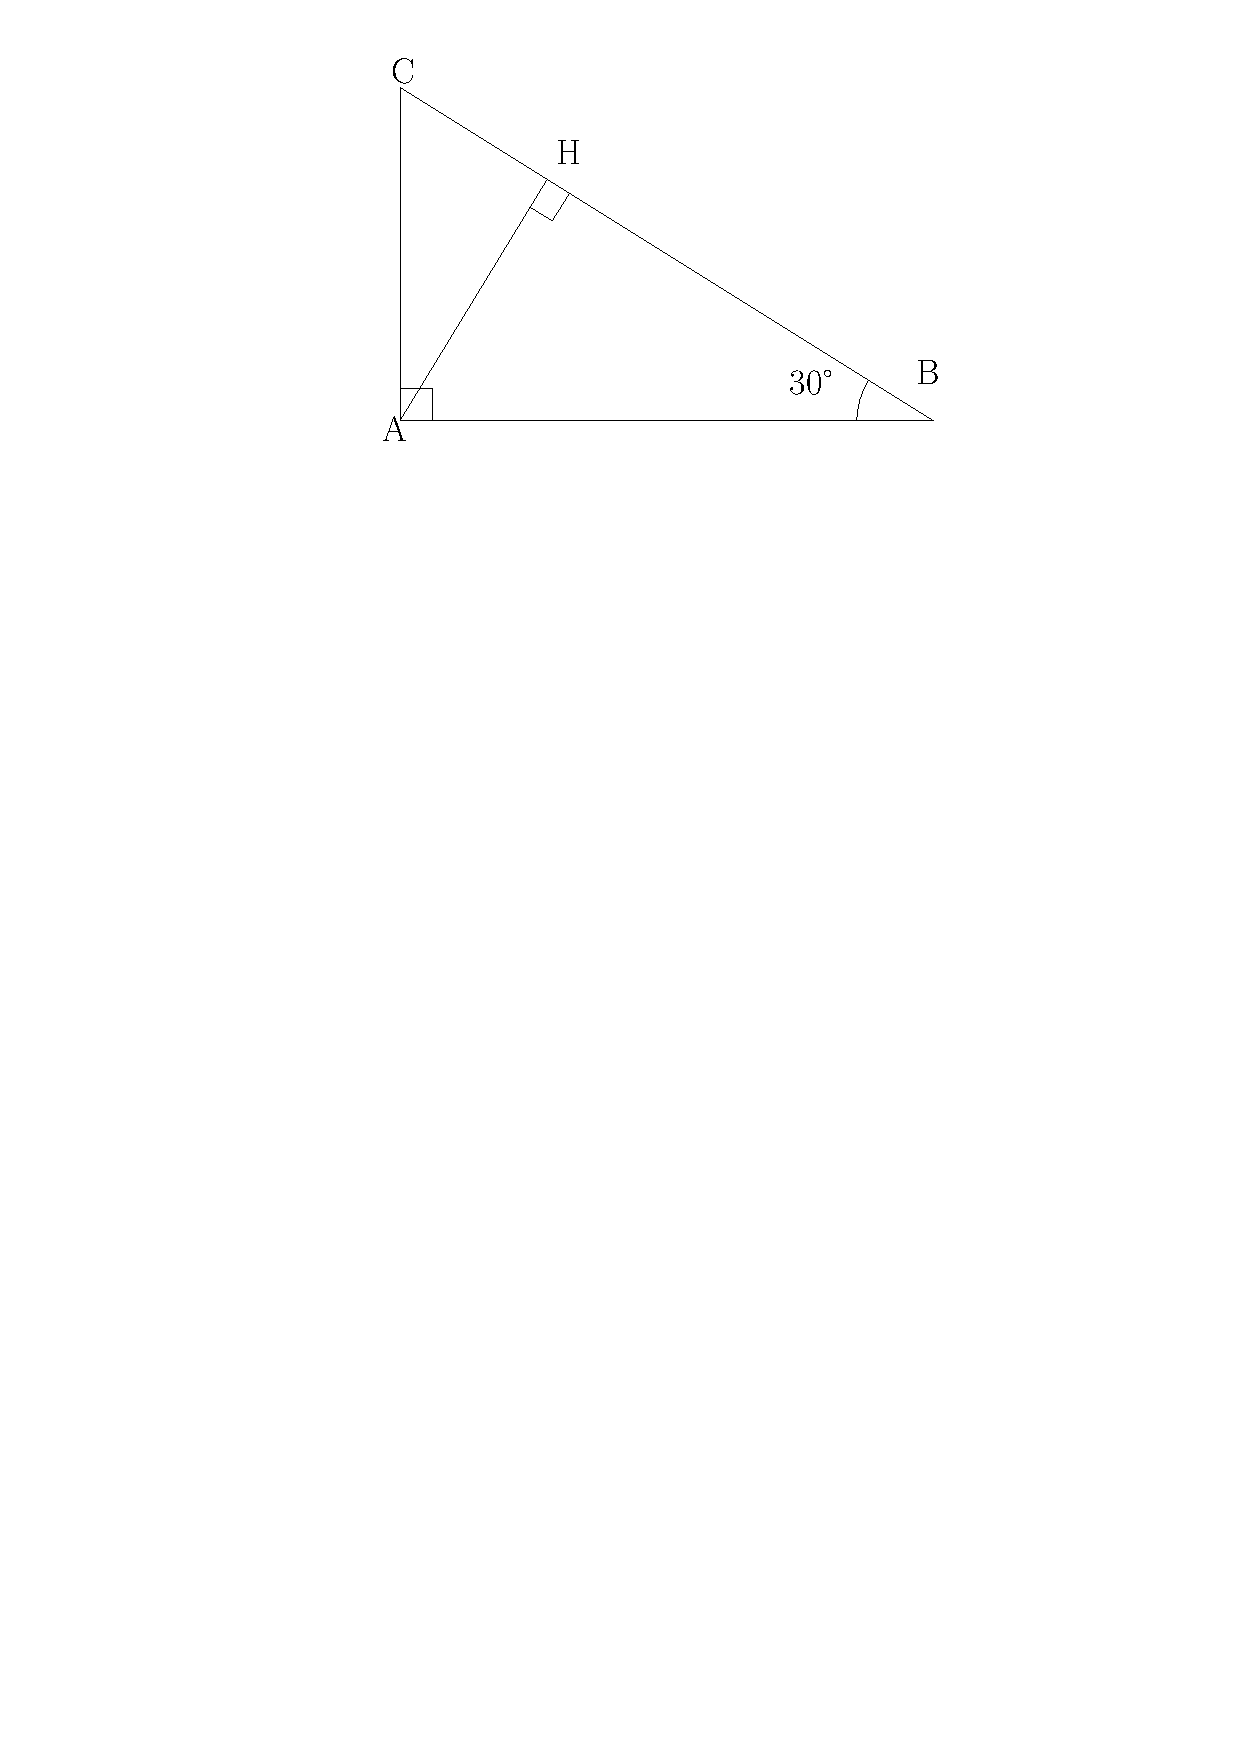
\includegraphics[width=100px]{4x10-trigonometrie/tri.pdf}
\end{figure}
\end{center}

\begin{enumerate}
  \item[1.] Remplir le tableau en calculant l'opposé en fonction de l'angle : $\alpha$.
  \item[2.] Tracer les courbes correspondantes à l'opposée et à l'adjacent en fonction de l'angle : $\alpha$.
\end{enumerate}

\subsection*{Calcul des angles}

\begin{enumerate}
  \item[1.] On sait que l'adjacent est égal à 800, lire la valeur de l'angle  : $\alpha = $ \dotfill
  \item[2.] À l'aide de la calculatrice, appuyer sur la touche seconde puis $\cos$ pour voir apparaître une nouvelle fonction : \dotfill
  \item[3.] Calculer $800 \div 1000 = $ \dotfill
  \item[4.] Calculer $\arccos(0,800) = $ \dotfill
\end{enumerate}
\end{minipage}

\begin{center}
\begin{tikzpicture}[yscale=2,xscale=2]
  \begin{axis}%
    [grid=both,
     minor tick num=1,
     grid style={line width=.1pt, draw=gray!30},
     major grid style={line width=.2pt,draw=gray!90},
     axis lines=middle,
     xmin=0,xmax=90,ymin=0,ymax=1000,
     xtick={5,10,15,20,25,30,35,40,45,50,55,60,65,70,75,80,85,90},
     xticklabels={5°,10°,,20°,,30°,,40°,,50°,,60°,,70°,,80°,,90°},
     ytick={0,100,200,300,400,500,600,700,800,900,1000},
     yticklabels={0,100,200,300,400,500,600,700,800,900,1000}
    ]
  \end{axis}
\end{tikzpicture}
\end{center}

\textbf{Les fonctions arccos et arcsin permettent de \dotfill }

\end{document}
